\documentclass[draftthesis,tocnosub,noragright,centerchapter,12pt]{uiucecethesis09} 
% Use draftthesis for notes and date markings on every page.  Useful when you
%   have multiple copies floating around.
% Use offcenter for the extra .5 inch on the left side. Needed with fullpage and fancy.
% Use mixcasechap for compatibility with hyperref package, which does NOT like all caps default
% Use edeposit for the adviser/committee on the title page.
% Use tocnosub to suppress subsection and lower entries in the TOC.
% PhD candidates use "proquest" for the proquest abstract.

\makeatletter

\usepackage{setspace}
\usepackage{epsfig}  % for figures
%\usepackage{graphicx}  % another package that works for figures
%\usepackage{subfigure}  % for subfigures
\usepackage{amsmath}  % for math spacing
%\usepackage{amssymb}  % for math spacing
%\usepackage{url}  % Hyphenation of URLs.
\usepackage{lscape}  % Useful for wide tables or figures.
\usepackage[justification=raggedright]{caption}	% makes captions ragged right - thanks to Bryce Lobdell
\usepackage{standalone}
% Tikz package
\usepackage{tikz}
\usetikzlibrary{arrows}
% My settings
\usepackage{mythesis}

% Uncomment the appropriate one of the following four lines:
%\msthesis
%\phdthesis
%\otherdoctorate[abbrev]{}
\college{College} % Replace 'Graduate College'
\othermasters{Bachelor of Science}{B.S.}

\title{Microphone Array Processing Techniques For Automatic Lecture Monitoring}
\author{Adam Miller}
\department{Electrical and Computer Engineering}
\degreeyear{2014}

% Advisor name is required for
% - doctoral students for the ProQuest abstract
% - master's students who do not have a master's committee
\advisor{Paris Smaragdis}

% Uncomment the \committee command for
% - all doctoral students
% - master's students who have a master's committee
%\committee{Professor Firstname Lastname, Chair\\
%        Professor Firstname Lastname} % etc.

\begin{document}

%%%%%%%%%%%%%%%%%%%%%%%%%%%%%%%%%%%%%%%%%%%%%%%%%%%%%%%%%%%%%%%%%%%%%%%%%%%%%%%
% COPYRIGHT
%
%\copyrightpage
%\blankpage

%%%%%%%%%%%%%%%%%%%%%%%%%%%%%%%%%%%%%%%%%%%%%%%%%%%%%%%%%%%%%%%%%%%%%%%%%%%%%%%
% TITLE
%
\maketitle

%\raggedright
\parindent 1em%

\frontmatter

%%%%%%%%%%%%%%%%%%%%%%%%%%%%%%%%%%%%%%%%%%%%%%%%%%%%%%%%%%%%%%%%%%%%%%%%%%%%%%%
% ABSTRACT
%
\begin{abstract}
% Put the abstract in a file called "abs.tex" and it'll be inputted here.
%\documentclass{article}

%\begin{document}
Here is my wondefully crafted abstract
%\end{document}

\end{abstract}


%%%%%%%%%%%%%%%%%%%%%%%%%%%%%%%%%%%%%%%%%%%%%%%%%%%%%%%%%%%%%%%%%%%%%%%%%%%%%%%
% DEDICATION
%
\begin{dedication}
% Whatever dedication you want.
To my parents, for their love and support.
\end{dedication}

%%%%%%%%%%%%%%%%%%%%%%%%%%%%%%%%%%%%%%%%%%%%%%%%%%%%%%%%%%%%%%%%%%%%%%%%%%%%%%%
% ACKNOWLEDGMENTS
%
% Put acknowledgments in a file called "ack.tex" and it'll be inputted here.
\begin{acknowledgments}
Here are all my acknowledgments

\end{acknowledgments}

%%%%%%%%%%%%%%%%%%%%%%%%%%%%%%%%%%%%%%%%%%%%%%%%%%%%%%%%%%%%%%%%%%%%%%%%%%%%%%%
% TABLE OF CONTENTS
%
\tableofcontents

%%%%%%%%%%%%%%%%%%%%%%%%%%%%%%%%%%%%%%%%%%%%%%%%%%%%%%%%%%%%%%%%%%%%%%%%%%%%%%%
% LIST OF TABLES
%
% The List of Tables is not strictly necessary. Omitting the List of Tables will
% simplify the thesis check and reduce the number of corrections.
\listoftables

%%%%%%%%%%%%%%%%%%%%%%%%%%%%%%%%%%%%%%%%%%%%%%%%%%%%%%%%%%%%%%%%%%%%%%%%%%%%%%%
% LIST OF FIGURES
%
% The List of Figures is not strictly necessary. Omitting the List of Figures will
% simplify the thesis check and reduce the number of corrections.
\listoffigures

%%%%%%%%%%%%%%%%%%%%%%%%%%%%%%%%%%%%%%%%%%%%%%%%%%%%%%%%%%%%%%%%%%%%%%%%%%%%%%%
% LIST OF ABBREVIATIONS
%
% The List of Abbreviations is not strictly necessary.
\chapter{LIST OF ABBREVIATIONS}

%\begin{symbollist*}
%\item[EPIC] Explicitly Parallel Instruction Computing
%\item[GPU] Graphics Processing Unit
%\item[VLIW] Very Long Instruction Word
%\end{symbollist*}


%%%%%%%%%%%%%%%%%%%%%%%%%%%%%%%%%%%%%%%%%%%%%%%%%%%%%%%%%%%%%%%%%%%%%%%%%%%%%%%
% LIST OF SYMBOLS
%
%\begin{symbollist}[0.7in]
%\item[$\tau$] Time taken to drink one cup of coffee.
%\end{symbollist}

\mainmatter

%%%%%%%%%%%%%%%%%%%%%%%%%%%%%%%%%%%%%%%%%%%%%%%%%%%%%%%%%%%%%%%%%%%%%%%%%%%%%%%
% INSERT REAL CONTENT HERE
%
\documentclass{uiucecethesis09} 

\usepackage{standalone} 

\begin{document}
\chapter{Introduction}

This chapter will discuss some of the motivation behind this project, as well as
the goals and distinguishing features of the project. The value of automated
lecture recording as a whole will be described, and an overview will be given of
the techniques to be presented in the remainder of the thesis.

\section{Overview} 

  \subsection{Motivation}

    In the last decade or so, the availability of online educational resources
    has increased significantly. With the launch of MIT OpenCourseWare over 10
    years ago and the now growing popularity of Massive Open Online Courses, the
    internet has become a substantive educational outlet. Additionally, much of
    this media is comprised of lectures given in classrooms or auditoriums to
    real audiences, that have also been recorded and uploaded. Because of this,
    systems for efficiently recording and processing such lectures have become
    more and more important.

    Yet the benefits of such systems can be seen even for students who attend the
    schools holding the lectures. In fact, many times such students are the main
    consideration for these systems, since the availability of a lecture online
    allows students to review that lecture at a later time \cite{bibs}. This can
    free students from the burden of capturing all the material during the actual
    lecture and may allow them to focus more heavily on the concepts being discussed
    rather than writing it down for review later.  

    As it stands, there is a lot that goes into processing many of the open lecture
    resources available online. In addition to ensuring a quality recording of the
    lecture, there is a certain amount of editing and post-processing that usually
    must occur \cite{passivecapture}. Some of this is to improve the flow of the
    material for the end viewer, but some of this may also involve dealing with
    mistakes made by those responsible for filming the lectures. In fact, it has
    been shown that even systems that are not fully automated enjoy better quality
    filming when the filming is attempted automatically and merely monitored by an
    operator (TODO cite).

    In addition to the time saving qualities of automated filming, such techniques
    can also provide substantial cost savings. While the cost of the necessary
    technology for these systems is continually decreasing, the cost of employing a
    person to record and edit the lectures is not. Because of this, prices reported
    for upkeep in such processes can be quite high \cite{Liu:2001}, making any
    opportunity for automation an opportunity for savings as well.  Beyond this,
    because automation can lower costs of producing such media, certain material may
    now be recorded and made available that would not have previously warranted it
    \cite{Bianchi:AVP}. This can help to continue the growth of online media and
    further propel the positive affects of such efforts. 

  \subsection{Focus}
    
    Automatic lecture monitoring as it has been described clearly can involve
    many separate phases. First the lecturer must take any necessary actions to
    initiate the lecture recording. Depending on the system, this may involve
    wearing a certain device to enable tracking, setting up the proper recording
    equipment, or simply pressing some button on a provided interface to
    initiate an automated process. Much of this depends on whether the system is
    designed to be passive or not - that is, whether or not the recorder needs
    to act any differently simply because the lecture is being recorded
    \cite{passivecapture}. 

    In the next step the lecture must actually be recorded -- both in video and
    audio. Again, depending on whether the system is a passive recording system or
    not, this can range from requiring no additional action, to requiring the
    lecturer to take certain actions throughout the presentation to ensure proper
    execution of the monitoring system.

    Finally, there is often a certain amount of post-processing that occurs in order
    to refine the recording.  This can include aligning supplementary materials with
    the video recording, or perhaps slicing up the recording into smaller clips.
    Some systems aim to do this automatically \cite{passivecapture}, but many do
    not.

    Despite the extent of this entire process, in this work we will focus solely on
    the first aspect of this process: the recording of the speaker. More
    specifically, the focus will be on passive recording techniques that utilize
    microphone array processing for locating and tracking the speaker. A camera will
    then be used to film the speaker once the correct location has been determined. 

    In most automated lecture capture systems, computer vision methods are used 
    on the video feeds to track the speaker \cite{Bianchi:AVP},
    \cite{Zhang05anautomated}, \cite{chou:2010}, \cite{Liu:2001}. Microphone arrays
    are then used to locate audience members asking questions, but are not involved
    in the tracking of speakers on stage \cite{Liu:2001}, \cite{Zhang05anautomated}.
    However, microphone array processing techniques could allow for localization of
    the speaker as well, and could help to add robustness to a video tracking system
    by providing additional information.  Moreover, since many systems employing
    computer vision tracking methods have at least two separate cameras -- one for
    following the speaker and one for recording the entire stage to detect movement
    \cite{Bianchi:AVP}, \cite{Liu:2001} -- by using a microphone array to perform
    much, if not all, of the speaker tracking it could be possible to eliminate one
    camera and cut down on the costs of such systems.

\end{document}
	% for INTRODUCTION in "intro.tex"
\documentclass{uiucecethesis09}
\usepackage{mythesis}

\begin{document}
\chapter{Background}
  \label{chap:background}

  To understand the techniques used in this project, it is necessary to 
  understand certain background material. Namely, what microphone arrays are and 
  what can be done with them. The techniques covered in this chapter will 
  heavily influence the material in later chapters and provide a foundation for 
  the work in the rest of the project.

  \section{Microphone Arrays}

    \subsection{Properties}
      In this project, we will use fixed microphone arrays, which are comprised 
      of a set of $\nmics$ microphones arranged in some fixed geometry. 

      A popular example of a microphone array is the equally spaced linear 
      array, which consists of $\nmics$ microphones in a line with a distance 
      $d$ between each consecutive microphone. An illustration of this is given 
      in \figref{fig:lin_mic_array}, and an example of such a system in 
      \figref{fig:ps3_eye}.  The popularity of this configuration comes from the 
      ease with which analysis can be performed due to the simplicity of the 
      geometry.  However, several other geometries are possible. A circular 
      microphone array is shown in \figref{fig:circle_array} and a three 
      dimensional 'cone' geometry is shown in \figref{fig:microcone}. In this 
      project we will make use of the PS3 Eye (shown in \figref{fig:ps3_eye}) 
      and the Dev Audio Microcone (shown in \figref{fig:microcone}) for our 
      experiments.

      % Linear Microphone Array Figure
      \begin{figure}[bottom]
        \begin{center}
          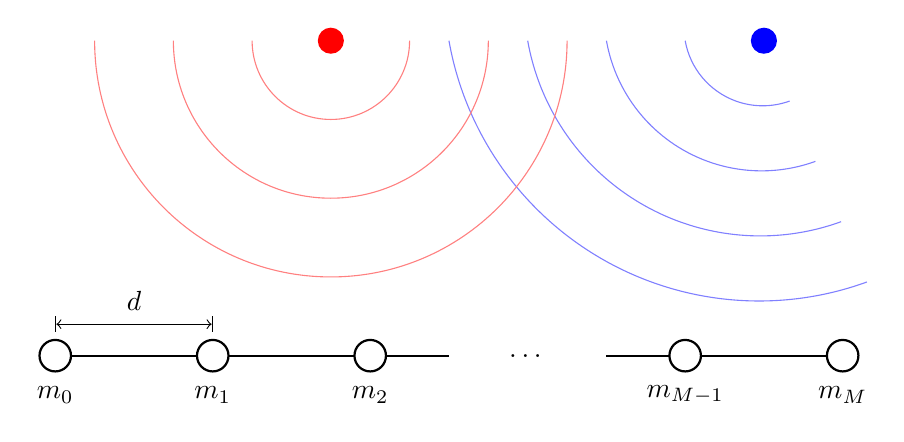
\begin{tikzpicture}
  [mic/.style={shape=circle, black, fill=white, thick, minimum size=4mm}]
  % Setup constants
  \def\miclineoffset{.4}
  \pgfmathsetmacro{\doffset}{\miclineoffset+.3}
  \pgfmathsetmacro{\miclabeloffset}{-.5}
  % Draw the lines on which the microphones will lie
  \draw [thick] (0,0) -- (5,0);
  \draw [thick] (7,0) -- (10,0);
  % Draw the first three mics in the group
  \draw [|<->|] (0,\miclineoffset) -- (2, \miclineoffset);
  \foreach \x in {0, 1, 2} {
    \node at (2*\x, 0) [mic, draw] {};
    \node at (2*\x, \miclabeloffset) {$m_{\x}$};
  }
  % Separator between sets of nodes
  \node at (6, 0) {\ldots};
  % Last few nodes that will be indexed from the end (M)
  \node at (8, 0) [mic, draw] {};
  \node at (8, \miclabeloffset) {$m_{M-1}$};
  \node at (10, 0) [mic, draw] {};
  \node at (10, \miclabeloffset) {$m_{M}$};
  \node at (1, \doffset) [] {$d$};

  % Draw arcs for sound waves
  \node[circle, fill=blue] at (9, 4) {};
  \foreach \rad in {1, 2, 3, 4} {
    \draw[blue!50] (9-\rad, 4) arc [start angle=190, end angle=290, 
    radius=\rad];
  }
  \node[circle, fill=red] at (3.5, 4) {};
  \foreach \rad in {1, 2, 3} {
    \draw[red!50] (3.5-\rad, 4) arc [start angle=180, end angle=360, 
    radius=\rad];
  }
\end{tikzpicture}

        \end{center}
        \caption{Linear microphone array configuration. Each microphone $m_\micidx$ 
        lies on a line and is separated from adjacent microphones by a distance 
      $d$.  There are two example sound sources.}
        \label{fig:lin_mic_array}
      \end{figure}

      % Examples of different microphone arrays
      \begin{figure}[b]
        \centering
        \begin{subfigure}[b]{.45\textwidth}
          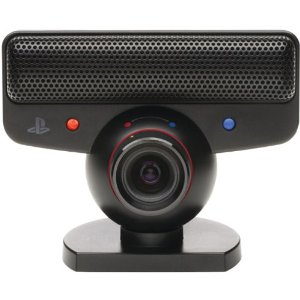
\includegraphics[width=\textwidth]{\thesisdir/background/figures/ps3_eye.jpg}
          \caption{PS3 Eye. Contains 4-microphone equidistance linear array}
          \label{fig:ps3_eye}
        \end{subfigure}
        \quad
        \begin{subfigure}[b]{.45\textwidth}
          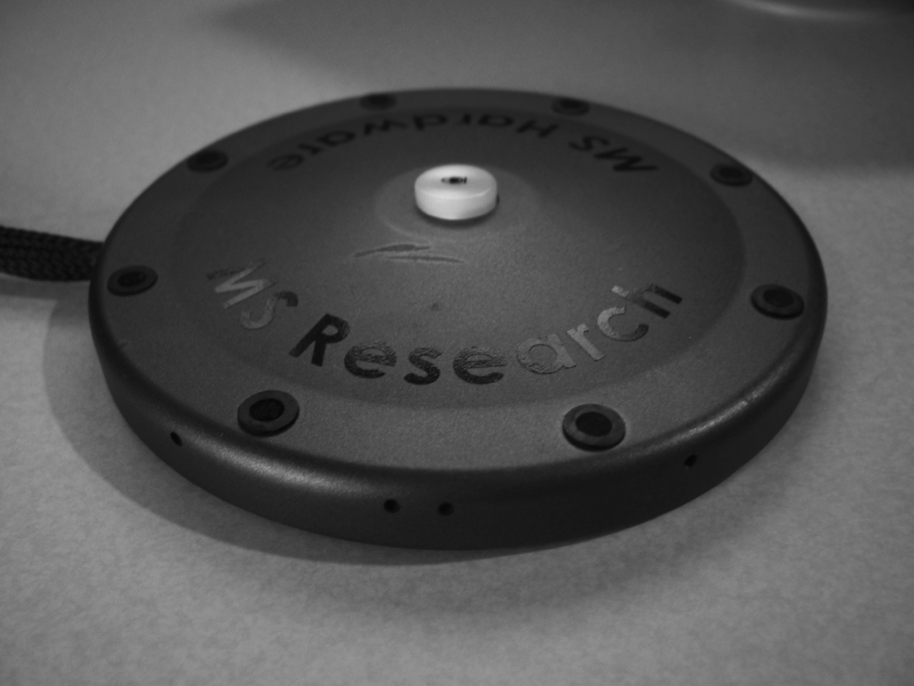
\includegraphics[width=\textwidth]{\thesisdir/background/figures/circle_array.png}
          \caption{ An eight-element circular microphone array 
            \cite{tashev2009sound}}
          \label{fig:circle_array}
        \end{subfigure}
        
        \begin{subfigure}[b]{\textwidth}
          \centering
          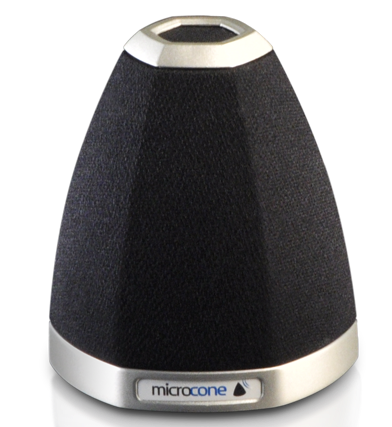
\includegraphics[width=.5\textwidth]{\thesisdir/background/figures/microcone.png}
          \caption{ The Dev Audio Microcone. This microphone array has six 
          microphones on the faces of a hexagonal base and one microphone at the 
        tip of the cone.}
          \label{fig:microcone}
        \end{subfigure}
        \caption{Microphone array examples}
        \label{fig:mic_array_examples}
      \end{figure}

      It may not be immediately apparent how a microphone array can provide any 
      advantage for processing signals. At each microphone we should expect to 
      hear the same signal with some delay, so how does this provide any 
      advantage?  
      
      One answer to this is that the signals will not be exactly the same at 
      each microphone; in fact, they will usually be corrupted by some noise in 
      the environment. The redundancy of the recordings can then be used to help 
      deduce what part of the signal is interesting, and what part of the signal 
      is noise. This is largely the focus of beamforming techniques and will be 
      reviewed in a later section
      
      However, even if the signals recorded at each microphone are just shifted 
      versions of the exact same source signal, there is still a gain to be had 
      from using multiple microphones. This is because by using a fixed 
      microphone array, one has infused the samples with spatial information -- 
      the information inherent in the spatial geometry of the array. In fact, 
      because of this it is possible to find the directivity of an array by 
      using the spatial Fourier transform \cite{benesty2010microphone}. It is 
      possible to use this property to infer spatial information about the 
      source.

    \subsection{Setup}
      \label{sec:setup}
      Consider a microphone array composed of $\nmics$ microphones with 
      microphone $\micidx$ located at position $\vect{\micpos}_\micidx$. Take the position 
      matrix $\mat{P}$ to be the matrix whose columns are composed of the 
      positions of the microphones:

      % Draw Position matrix
      \begin{equation} \label{eq:pos_mat}
        \mat{\posmat} =
          \begin{bmatrix} | & | && | \\
            \micpos_1 & \micpos_2 & \ldots & \micpos_\nmics \\
              | & | && |
          \end{bmatrix}
      \end{equation}

      Assume that there is some source signal $\srcsig(t)$ emanating from a 
      point source at position $\vect{\srcpos}$. Furthermore, assume that 
      $\vect{\srcpos}$ is far enough from each microphone that the far field 
      assumption holds. That is, the sound wave can be viewed as a plane wave 
      associating each microphone from the same direction. See TODOFIGURE for an 
      illustration. 
      
      Now select one of the microphones to be used as reference for the others.  
      We choose the first microphone.  It is possible to calculate the amount of 
      time it takes the sound signal to reach the reference microphone
      % Mic delays
      \begin{equation} \label{eq:ref_delay} \refdelay = \frac{\norm{\srcpos - 
        \micpos_1}}{\speedsound} \end{equation}
      where $\speedsound$ is the speed of sound.  In addition to this, we can 
      calculate the amount of time it takes for the sound to travel between the 
      reference microphone and any other microphone.  To do this we make use of 
      the far field model \cite{dudgeon1977fundamentals}.  Assume the sound wave 
      is a plane wave and $\srcdir$ is a unit vector pointing in the direction 
      of the sound source as viewed by the center of the microphone array. We 
      then have that
      \begin{equation} \label{eq:TDOA} \micdelay_\micidx = \frac{\left(\micpos_1 
        - \micpos_\micidx\right) \cdot \srcdir}{\speedsound} \end{equation}
      where $\micdelay_\micidx$ is the delay between the arrival of the signal 
      at microphone 1 and the arrival of the signal at microphone $\micidx$.  
      This is known as a time difference of arrival (TDOA).  This gives 
      \begin{align} \label{eq:mic_signal}
        \micrec_\micidx\oftime &= \atten_\micidx\srcsig\of{\sigtime - \refdelay - 
        \micdelay_\micidx} + \micnoise_\micidx\oftime\\
        &= \micsig_\micidx\oftime + \micnoise_\micidx\oftime
      \end{align}
      where $\micrec_\micidx\oftime$ is the signal recorded at microphone $\micidx$, 
      $\srcsig\oftime$ is the unknown source signal, $\alpha_\micidx$ are the 
      attenuation factors, and $\micnoise_\micidx\oftime$ are the additive noise heard 
      at each microphone.

      From this equation we see that if we assume all $\atten_\micidx$ are equal 
      we have
      \begin{equation} \label{eq:sig_shift} \micsig_\micidx\oftime = 
        \micsig_1\of{\sigtime - \micdelay_\micidx} \end{equation}
      which reaffirms the intuitive notion that the signal recorded at each 
      microphone will be just a shifted (and likely distorted) version of the 
      signal occurring at the reference microphone.
      
  \section{Beamforming}

    \subsection{Array Directivity}
      In \eqref{eq:sig_shift} we saw that each signal is just a shifted version 
      of the signal at the first microphone. In turn if we want to align the 
      signals we need only reverse such a shift. To do so we transfer our focus 
      to the frequency domain.
      The frequency domain equivalent of \eqref{eq:sig_shift} gives the 
      following
      \begin{equation} \label{eq:freq_shift} \Micsig_\micidx\offreq = 
        \Micsig_1\offreq e^{-j2\pi\freq\micdelay_\micidx}
        \end{equation}
      Now take the vector
      \begin{equation} \label{eq:steering_vec}
        \steer\of{\dir, \freq} =
        \begin{bmatrix} e^{j2\pi\freq\micdelay_1\of{\dir}} & 
          e^{j2\pi\freq\micdelay_2\of{\dir}} & \cdots & 
          e^{j2\pi\freq\micdelay_\nmics\of{\dir}}
        \end{bmatrix}\trans
      \end{equation}
      which can be seen to contain the opposite shifts for each microphone. Note 
      that here $\micdelay_\micidx$ has been written as a function of $\dir$ to 
      emphasize the dependence of the delays on a given steering direction. Now 
      if we look at the vector
      \begin{equation}
        \Micsig\offreq = \begin{bmatrix} \Micsig_1\offreq & \Micsig_2\offreq 
          & \cdots & \Micsig_\nmics\offreq \end{bmatrix}\trans
      \end{equation}
      we see that the vector product
      \begin{align}
        \steer\of{\dir, \freq}\trans \Micsig\offreq &= 
        \sum\limits_{\micidx=1}^{\nmics} \Micsig_\micidx\offreq 
        e^{j2\pi\freq\micdelay_\micidx\of{\dir}} \\
        &= \sum\limits_{\micidx=1}^{\nmics} \Micsig_\micidx\offreq 
        e^{j2\pi\freq\frac{\left(\micpos_1 - \micpos_\micidx\right) \cdot 
        \dir}{\speedsound}} \\
        &= \sum\limits_{\micidx=1}^{\nmics} \Micsig_\micidx\offreq 
        e^{-j2\pi\freq\frac{\left(\micpos_\micidx - \micpos_1\right) \cdot 
        \dir}{\speedsound}} \\
        &= \sum\limits_{\micidx=1}^{\nmics} \Micsig_\micidx\offreq 
        e^{-j2\pi\vect{\xi} \cdot \left(\micpos_\micidx - \micpos_1\right)}
      \end{align}
      equates to a spatial Fourier Transform, where
      \begin{equation} \vect{\xi} = \frac{\freq\dir}{\speedsound} \end{equation}
      is the spatial frequency vector. Just as a spectral Fourier Transform can 
      be interpreted as determining the energies in each constituent frequency 
      of a signal, this spatial Fourier Transform can be viewed as determining 
      the energies in each constituent direction of the signal, given a specific 
      frequency of the signal. This makes sense as here we sample the signal 
      across space where as in the spectral version we do so across time.

      Note however that the above equations were written assuming a fixed source 
      direction, $\srcdir$. In reality, the directivity is also a function of 
      the source direction as we have
      \begin{equation} \Micsig_\micidx\of{\srcdir, \freq} = \Micsig_1\offreq
        e^{-j2\pi\freq\micdelay_\micidx\of{\srcdir}} \end{equation}
      giving us the complete directivity
      \begin{align}
        \direct\of{\dir, \srcdir, \freq} &= \steer\of{\dir, \freq}\trans 
        \Micsig\of{\srcdir, \freq}\\
        &= \sum\limits_{\micidx=1}^{\nmics} \Micsig_\micidx\of{\srcdir, \freq}
          e^{-j2\pi\vect{\xi} \cdot \left(\micpos_\micidx - \micpos_1\right)} \\
        &= \Micsig_1\offreq\sum\limits_{\micidx=1}^{\nmics} 
        e^{-j2\pi\freq\micdelay_\micidx\of{\srcdir}}
          e^{-j2\pi\vect{\xi} \cdot \left(\micpos_\micidx - \micpos_1\right)}
      \end{align}
      % TODO: PLOTS OF DIRECTIVITIES FOR DIFFERENT MICROPHONES

      What we have shown here is that by aligning the signals as if they came 
      from a certain direction and then combining them, we are able to attribute 
      an amount of the signal that came from that direction. That is, we perform 
      a spatial Fourier Transform. We now see an alternative explanation for the 
      same process and how it falls into the greater context of beamforming.

    \subsection{Delay and Sum Beamformer}

      In the previous section we found how to the determine the directivity of 
      an array as a function of a steering direction $\dir$, source direction 
      $\srcdir$, and frequency $\freq$.  Consider now the case where $\dir = 
      \srcdir$. If we steer the array in this direction, we see that we get

      \begin{align}
        \steer\of{\srcdir, \freq}\trans \Micsig\of{\srcdir, \freq} &= 
        \sum\limits_{\micidx=1}^{\nmics} \Micsig_\micidx\of{\srcdir, \freq}
          e^{j2\pi\freq\micdelay_\micidx\of{\srcdir}} \\
        &= \Micsigf{1} \sum\limits_{\micidx=1}^{\nmics} 
        e^{-j2\pi\freq\micdelay_\micidx\of{\srcdir}} 
        e^{j2\pi\freq\micdelay_\micidx\of{\srcdir}} \\
        &= \nmics \Micsigf{1}
      \end{align}

      Which is just the signal at the reference microphone multiplied by the 
      number of microphones in the array.

      We can of course view this as simply summing all the recorded signals 
      after shifting them the correct amount to offset the propagation delay. If 
      we do this with the raw recorded signals and average the result we get

      \begin{align}
        \filtered\oftime &= \frac{1}{\nmics}\micsum \micrec_\micidx\of{\time + 
        \micdelay_\micidx}\\
        &= \frac{1}{\nmics}\micsum \atten_\micidx\micsig_\micidx\of{\time + 
        \micdelay_\micidx} + \frac{1}{\nmics}\micsum \micnoise_\micidx\of{\time 
        + \micdelay_\micidx}\\
        &= \atten\srcsig\of{\time - \refdelay} + \frac{1}{\nmics}\micsum 
        \micnoise_\micidx\of{\time + \micdelay_\micidx}
      \end{align}
      where
      \begin{equation}
        \atten = \frac{1}{\nmics}\micsum\atten_\micidx
      \end{equation}

      Quite appropriately, this is known as the delay and sum method for 
      beamforming \cite{benesty2010microphone}, \cite{dudgeon1977fundamentals}, 
      \cite{tashev2009sound}. In cases where the $\micnoise_\micidx\oftime$ are 
      uncorrelated, it can increase the SNR by a factor of $\nmics$, as a result 
      of the averaging across channels. However, in the case where the noise at 
      the microphones are correlated, the noise reduction decreases and with 
      perfect correlation is nonexistent \cite{benesty2010microphone}.

      The delay and sum method is the most straightforward of a variety of 
      beamforming approaches, all of which aim to use information available in 
      the signal recordings to reduce unwanted noise.

      %\begin{equation}
      %  \sum\limits_\micidx=0^{\nmics} 
    
\end{document} 

\documentclass{uiucecethesis09}
\usepackage{mythesis}

\begin{document}
\chapter{Direction of Arrival Estimation and Stateless Tracking}
  
  This chapter will explore the direction of arrival estimation methods as they 
  were implemented in our system. It will also describe how these estimates were 
  used to perform stateless tracking of speakers. By stateless, we refer to the 
  lack of a state dynamics model for the system or the maintenance of any such 
  external state that would allow for a prediction of the next state. We 
  nevertheless explore methods for smoothing our tracking estimates using 
  alternative approaches.

  \section{Direction of Arrival Estimation}
    We first consider methods for estimating the direction of arrival (DOA) of a 
    sound. As described in \secref{sec:setup}, this equates to estimating the 
    TDOA values given by \eqref{eq:TDOA}.
    \subsection{GCC-PHAT}
      The first method we describe is the Generalized Cross Correlation method 
      \cite{knapp1976generalized}, \cite{brandstein1997robust}, 
      \cite{benesty2010microphone}.
      We seek to find
      \begin{equation} \label{eq:gcc_estimate}
        \hat{\micdelay}_{\micidx, \micjdx} = \argmax_{\micdelay}{\gcc_{\micidx, 
        \micjdx}\of{\micdelay}} \end{equation}
      where
      \begin{align} \label{eq:gcc_dfn}
        \gcc_{\micidx,\micjdx}\of{\micdelay} &= 
        \int\limits_{-\infty}^{\infty}{\gccweightf\Micrec_\micidx^*\offreq\Micrecf{\micjdx} 
        e^{j2\pi\freq\micdelay}} d\freq\\
        %&= \int\limits_{\time^\prime}^{\time^{\prime} + \window} 
        %\micrec_\micidx\of{\time - \micdelay}\micrect{\micjdx} d\time \\
      \end{align}
      is the generalized cross correlation (GCC) function between microphone 
      $\micidx$ and microphone $\micjdx$. Here $\gccweightf$ is a spectrum 
      weighting function that can be used to scale the signal spectra and 
      improve the accuracy of the resulting TDOA estimate. This can be 
      interpreted as an additional set of filters through which the signals pass 
      that can help shape them for better estimation 
      \cite{brandstein1997robust}, \cite{knapp1976generalized}.  We see that for 
      a unity weighting function the GCC is equivalent to the standard cross 
      correlation function

      \begin{align}
        \cc_{\micidx, \micjdx}\of{\micdelay} &= \infint 
        \Micrec_\micidx^*\offreq\Micrecf{\micjdx} e^{j2\pi\freq\micdelay} 
        d\freq\\
        &= \infint \micrec_\micidx\of{\time - \micdelay} \micrect{\micjdx} 
        d\time 
        \label{eq:cc}
      \end{align}

      A variety of weighting functions are available 
      \cite{benesty2010microphone}, \cite{knapp1976generalized}, 
      \cite{brandstein1997robust}, however one of the most popular is the phase 
      transform (PHAT) weighting
      \begin{equation}
        \gccweight_{\text{PHAT}}\of{\freq}= 
        \frac{1}{\abs{\Micrec_\micidx^*\offreq\Micrecf{\micjdx}}}
        \label{eq:phat}
      \end{equation}
      which has been shown to be quite robust in noisy and reverberant 
      environments \cite{omologo93useof}. The combination of the generalized 
      cross correlation method with the phase transform weighting is referred to 
      as GCC-PHAT.

    \subsection{Point Estimates}
      Using the GCC-PHAT method, we can obtain a set of $\tdoaest_{\micidx, 
      \micjdx}$ values by searching for a peak in the resulting GCC function of 
      each necessary microphone pair. This set comprises our TDOA estimates.  
      From this, using \eqref{eq:TDOA} we can set up the following system.
      \begin{equation}
      \frac{1}{\speedsound} \begin{bmatrix} \micpos_1 - \micpos_2 \\ \micpos_1 - 
        \micpos_3 \\ \ \vdots \\ \micpos_1 - \micpos_\nmics \end{bmatrix} 
      \hat{\srcdir} = \begin{bmatrix} \tdoaest_{2} \\
        \tdoaest_{3} \\ \vdots \\ \tdoaest_{\nmics}\end{bmatrix}
      \label{eq:gcc_least_squares}
      \end{equation}
      with
      \begin{equation}
        \tdoaest_{i} = \tdoaest_{1,i}
      \end{equation}
      to be consistent with notation in \eqref{eq:TDOA}. Note that we only 
      consider delays between microphone 1 and all others since other delays 
      become linearly dependent. The solution may be solvable if the number of 
      microphones is one more than the number of dimensions in the search space 
      and the microphones have an appropriate geometry CITE TODO.  Otherwise we 
      must use a least squares solution.

      However, this method has a few negatives. First off, by doing this we will 
      be getting point estimates for the direction of arrival with no measure of 
      likelihood. Therefore, we are making a hard decision about our estimate and 
      if this estimate is used in a larger system, we have made a great 
      commitment at an early stage. This should be avoided if at all possible.  
      Secondly, to actually implement this method we must discretize the 
      $\micdelay$ search space. In doing so, we are inherently discretizing the 
      search space of $\hat{\srcdir}$, which may end up leading to a 
      discretization that is inefficient or ineffective for our purposes.

      A remedy for the first problem could be to aggregate the correlation 
      values for each combination of discrete $\micdelay$ values. Then the 
      magnitude of these correlation values could be used as a likelihood score 
      as we will discuss later.  However, this would be extremely expensive 
      computationally, and in doing so we would be considering many infeasible 
      directions.  Yet, despite this problem, this method is not far off.  In 
      fact if we perform a similar calculation for only combinations of 
      $\micdelay_\micidx$ values that correspond to feasible search directions, 
      we can rectify both of the mentioned problems.

    \subsection{Likelihood Approach}
      As mentioned, the goal is to obtain a likelihood for each feasible 
      direction of arrival. We use methods similar to \cite{dmochowski2008fast}, 
      \cite{DiBiase00ahigh-accuracy}. Unfortunately the space of feasible 
      direction of arrivals is continuous and while attempts to create 
      continuous likelihood models over the search space based on TDOA estimates 
      exist \cite{brandstein1997closed}, we chose to instead discretize the 
      search space. By sampling our search space, we can now determine exactly 
      which TDOAs are of interest.  That is, for each feasible source direction 
      $\dir$ we can calculate $\micdelay_\micidx\of{\dir}$ for any microphone 
      $\micidx$.  We then need only compute the correlation values:
      \begin{align}
      \gcc_{\micidx, \micjdx}\of{\micdelay_\micjdx\of{\dir} - 
      \micdelay_\micidx\of{\dir}} &= \infint \gccweightf 
      \Micrec_\micidx^*\offreq\Micrecf{\micjdx}
      e^{j2\pi\freq\left(\micdelay_\micjdx\of{\dir} - 
      \micdelay_\micidx\of{\dir}\right)} d\freq \\
      \end{align}
      Now to get a likelihood score we average across the different channel 
      pairs, giving
      \begin{equation}
        \lhood_{\text{GCC}}\of{\dir} = \pairsum\shape\of{\gcc_{\micidx, 
        \micjdx}\of{\micdelay_\micjdx\of{\dir} - \micdelay_\micidx\of{\dir}}}
      \end{equation}
      where $\shape\of{x} = x^k$ is a likelihood shaping function, used to 
      sharpen peaks and reduce sidelobes \cite{ward2002particle}.  
      
      \begin{figure}[h]
        \centering
        \includegraphics[width=\textwidth]{figures/gcc_likelihoods.png}
        \caption{Normalized GCC Values for various values of $k$ in the shaping 
          function $\shape\of{x} = x^k$. We see the speak sharpen as the value 
        of $k$ increases from 1 to 5.}
        \label{fig:gcc_shapes}
      \end{figure}

    \subsection{Beamforming and SRP-PHAT}
      The method described is also sometimes referred to as SRP-PHAT (where SRP 
      stands for Steered Response Power)  when the PHAT weighting function is 
      used to calculate the GCC \cite{dmochowski2008fast}.  This results from 
      the fact that we are calculating the energy in the scaled Crosspower 
      spectrum \cite{omologo93useof} after steering the array in each feasible 
      direction $\dir$. This suggests that this method can be viewed in a 
      beamforming context.

      Consider using a delay and sum beamformer to steer the signal in each 
      feasible direction $\dir$ and then taking the power of the corresponding 
      signal. 

      \begin{align}
        \lhood_{\text{DS}}\of{\dir} &= \infint \left[\micsum 
        \micrec_\micidx\of{\time + \micdelay_\micidx\of{\dir}} \right]^2 d\time 
        \\
        &= \micsum \micsumk{\micjdx} \infint \micrec_\micidx\of{\time + 
          \micdelay_\micidx\of{\dir}} \micrec_\micjdx\of{\time + 
            \micdelay_\micjdx\of{\dir}} d\time \\
        &= \micsum \micsumk{\micjdx} \infint \micrec_\micidx\of{\time + 
          \micdelay_\micidx\of{\dir}-\micdelay_\micjdx\of{\dir} } 
          \micrec_\micjdx\oftime d\time
        \label{eq:srp_phat} \\
        &= \micsum \micsumk{\micjdx} \infint \Micrec_\micidx^*\offreq 
        \Micrecf{\micjdx} e^{j2\pi\freq\left(\micdelay_\micjdx\of{\dir} - 
        \micdelay_\micidx\of{\dir}\right)} d\freq \\
        &= 2\lhood_{\text{GCC}}\of{\dir} + \micsum \infint 
        \Micrec_\micidx^*\offreq\Micrecf{\micidx} d\freq
      \end{align}

      We see that if we use $\shape\of{x} = x$ and add in a weighting function 
      $\gccweightf$ we get that the result is equal to our earlier likelihood 
      plus the total signal energy. It can be shown that these two likelihood 
      scores are closely related to a Bayesian likelihood of the signal given 
      the prospective direction \cite{Birchfield02fastbayesian}.

      Just as a spectrum weighting function $\gccweightf$ was added with the GCC 
      method, a weighting function for combining frequencies can be added here . 
      While there again are various weighting functions, the phase transform is 
      often used, leading to the denomination of this method as SRP-PHAT 
      \cite{DiBiase00ahigh}. There also exist analogous SRP algorithms for 
      beamforming methods other than delay and sum.  Good coverage of these 
      methods is given in \cite{tashev2009sound}
      TODO FIGURE

  \section{Tracking}
    \subsection{Raw DOA Estimates}
      The most obvious
        
      






\end{document}

%\include{concl}


%%%%%%%%%%%%%%%%%%%%%%%%%%%%%%%%%%%%%%%%%%%%%%%%%%%%%%%%%%%%%%%%%%%%%%%%%%%%%%%
% APPENDIX
%
\appendix
%\include{apx}

\backmatter

%%%%%%%%%%%%%%%%%%%%%%%%%%%%%%%%%%%%%%%%%%%%%%%%%%%%%%%%%%%%%%%%%%%%%%%%%%%%%%%
% BIBLIOGRAPHY
%
\bibliographystyle{IEEE_ECE}
% Put references in BibTeX format in thesisrefs.bib.
\bibliography{thesisrefs}


%%%%%%%%%%%%%%%%%%%%%%%%%%%%%%%%%%%%%%%%%%%%%%%%%%%%%%%%%%%%%%%%%%%%%%%%%%%%%%%
% AUTHOR'S BIOGRAPHY
% As of 10/03/2011, Author's Biography or Vita no longer accepted by Grad College

\end{document}
\endinput
